The \verb+vga_drive+ module exists to handle the rendering of a 640x480 resolution image on the screen. 
The image that is supposed to be rendered consists of a background image previously 
stored in the SRAM consisting of pre filled bars that within the module will be blanked
out according to the input stimuli, which will give the appearance of bars being filled 
to different levels.   

To render an image on the vga screen you need five main signals. Three analog color channels (red, green and blue)
and two signals for synchronization hsync and vsync. The image is rendered pixel by pixel line by line using
a horizontal sweep pattern which is reset by the two sync signals. If a color is set when the sweep resets
arbitrary patterns can occur and therefore the signal has to be blanked during the reset phase.

The module \verb+vga_drive+ has four input signals described in 

\begin{figure}[h]
        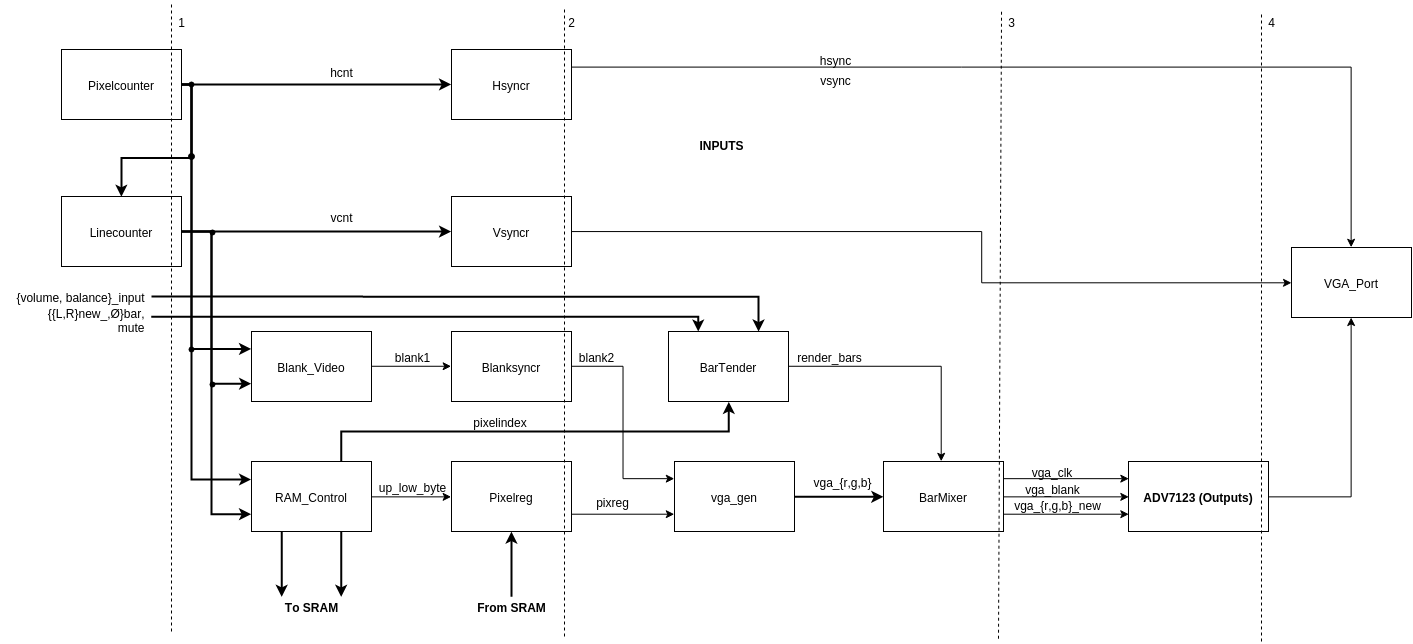
\includegraphics[scale=0.35]{vgadrive.png}
        \caption{Block diagram of vga\_drive}
        \label{fig:vgadrive}
\end{figure}

\begin{figure}[h]
        \caption{List of input signals}
        \label{tab:input}
\begin{tabular}{|r|l|}
        \hline
        \multicolumn{2}{|c|}{Input signals}\\
        \hline
        \multicolumn{1}{|c}{Name} & \multicolumn{1}{c|}{Description} \\
        \hline
        volume\_input & a 4 bit input containing volume information\\
        \cline{1-2}
        \hline
        balance\_input & a 4 bit input containing balance information\\
        \cline{1-2}    
        \hline
        bar & a n bit input containing signal sound input signal level\\
        \cline{1-2}    
        \hline
        new\_bar & a n bit input containing manipulated input signal level\\
        \cline{1-2}    
        \hline
\end{tabular}
\end{figure}

\begin{figure}[h]
        \caption{List of output signals}
        \label{tab:outputs}
\begin{tabular}{|r|l|}     
        \hline
        \multicolumn{2}{|c|}{output signals}\\
        \hline
        \multicolumn{1}{|c}{Name} & \multicolumn{1}{c|}{Description} \\
        \hline
        vga\_clk & clock signal needed for scanning\\
        \cline{1-2}
        \hline
        vga\_blank & a blanking signal for blanking when reseting scan\\
        \cline{1-2}    
        \hline
        vga\_(r,g,b) & three signals containing color information\\
        \cline{1-2}    
        \hline
\end{tabular}
\end{figure}

  \subsection{VGA\_driver:bartender}
  \subsection{VGA\_driver:barmixer}

